The search for $t\bar{t}H/A \to t\bar{t}t\bar{t}$ production in the 1L/2LOS final state presented in this article is combined with the ATLAS measurement in the 2LSS/3L final state using the same data set. 
The combination is performed via a simultaneous profile likelihood fit in all regions of both analysises, with all systematic uncertainties included, and the combined upper limit of $t\bar{t}H/A \to t\bar{t}t\bar{t}$ production cross section is extracted. 
The events in the two analysises are statiscally independent by construction due to the different lepton selection criteria.

\subsection{Correlation of systematic uncertainties}
\label{sub:combination_correlation}

The experimental uncertainties are treated as fully correlated between the two final states since both analysises use the same reconstructed objects and data set. 
Theoretical modelling uncertainties in the non-$t\bar{t}$ backgrounds and the BSM $t\bar{t}t\bar{t}$ signal are also correlated if they have identical definition at both 1L/2LOS and 2LSS/3L final states except for those related to $t\bar{t}W$ background,which is treated differently in the 1L/2LOS and 2LSS/3L final states. In the latter, $t\bar{t}W$ is the most important background and a detailed systematics model has been studied, while in the former it is a small background.
The uncertainties related to the modelling of the $t\bar{t}$+jets background are treated as uncorrelated between the 1L/2LOS and 2LSS/3L final states. In account of the contribution of $t\bar{t}$+jets events in the 2LSS/3L final state is much smaller than that in the 1L/2LOS final state, and arises from misreconstructed or non-prompt leptons, while it is the dominant irreducible background in the 1L/2LOS final state. Its estimation and the treatment of relevant uncertainties is therefore different in the two final states. 
The systematic uncertainties associated with the reducible backgrounds in the 2LSS/3L final state and uncertainties related to the data-driven corrections to the $t\bar{t}$+jets background in the 1L/2LOS final state are uncorrelated.

\subsection{Combined data fit}
\label{sub:combination_fit}

The combined fit to unblinded data is performed as a simultaneous fit in all analysis regions from both channels with all systematic uncertainties included and the correlations treated as described in Section \ref{sub:combination_correlation}.
Figure \ref{fig:combination_limit_1} show the observed and expected upper limit of $t\bar{t}H/A \to t\bar{t}t\bar{t}$ production cross section, also with the comparison of the expected upper limit among each separated channels and the combined fit.
Exclusion limit of $\tan\beta$ as a function of $m_{H/A}$ is shown in Figure \ref{fig:combination_2Dplots}.
Figure \ref{fig:combination_limit_2} show the comparison of the observed and expected upper limit of $t\bar{t}H/A \to t\bar{t}t\bar{t}$ production cross section between the combined fit and each separated channel.

The expected and observed significances of $t\bar{t}H/A \to t\bar{t}t\bar{t}$ production are shown in Figure \ref{fig:combination_significance}, with comparison among each separated channels and the combined fit.
The fitted signal strength comparison among each separated channels and the combined fit is shown in Figure \ref{fig:combination_mu}
The nuisance paremeter pulls comparison among the combined fit and each channel fit of mass point 400 GeV, 700 GeV and 1000 GeV are shown in figure \ref{fig:combination_NP}. Pulls and constraints of the detector uncertainties in the combined fit mostly follow the ones observed in the 1LOS channel.
The combined correlation matrix of mass point 400 GeV is shown in figure \ref{fig:combination_CorrMatrix}. Large correlation with $\mu$ is observed for $t\bar{t}t\bar{t}$ modelling systematics.

95\% CL upper limit on the cross section of $t\bar{t}H/A \to t\bar{t}t\bar{t}$ production ranged between 15.288 fb and 5.0856 fb for a heavy Higgs boson mass between 400 GeV and 1000 GeV, respectively.


\begin{figure}[htbp!]
    \centering
    \begin{subfigure}[t]{0.49\textwidth}
      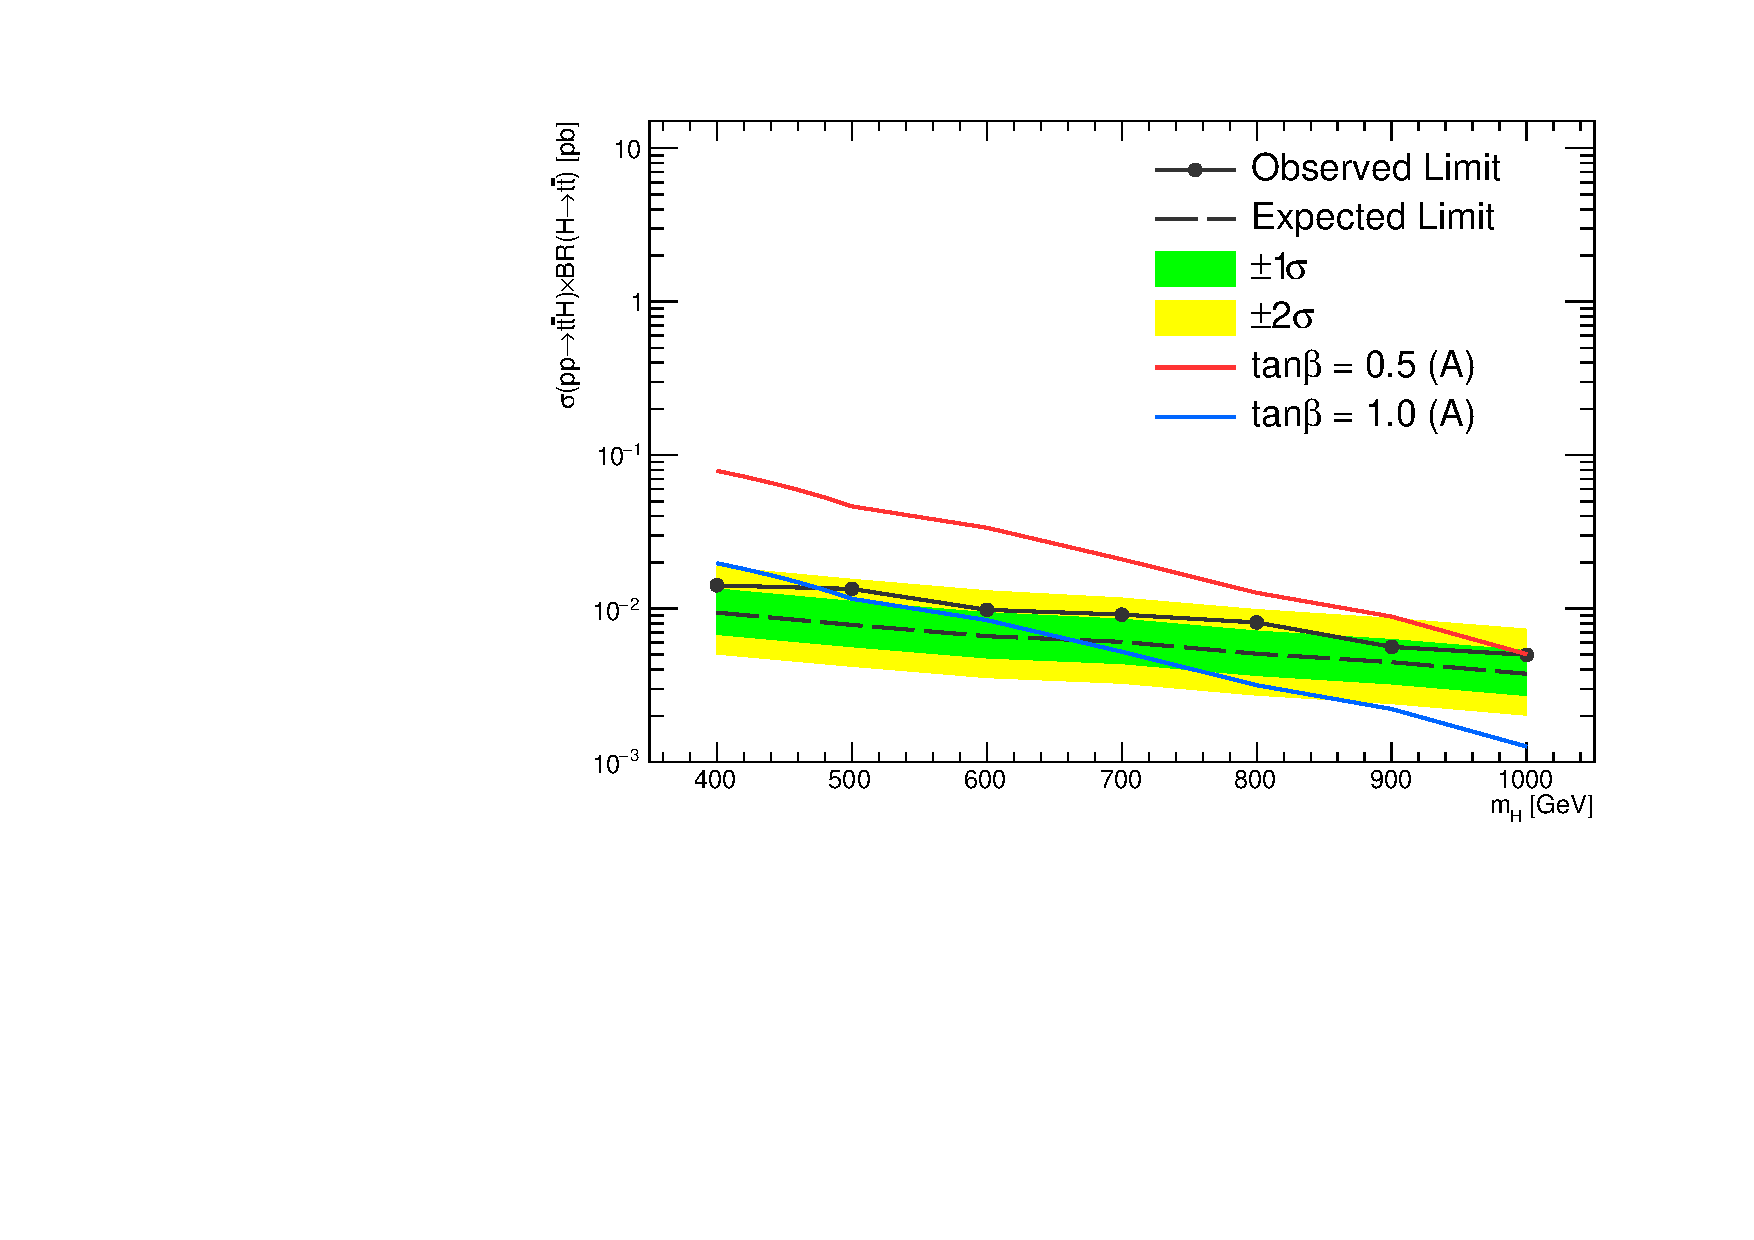
\includegraphics[width=1 \textwidth]{figures/combined_fit/lim_combined.pdf}
      \caption{Expected and observed limits}
    \end{subfigure}
    \begin{subfigure}[t]{0.49\textwidth}
      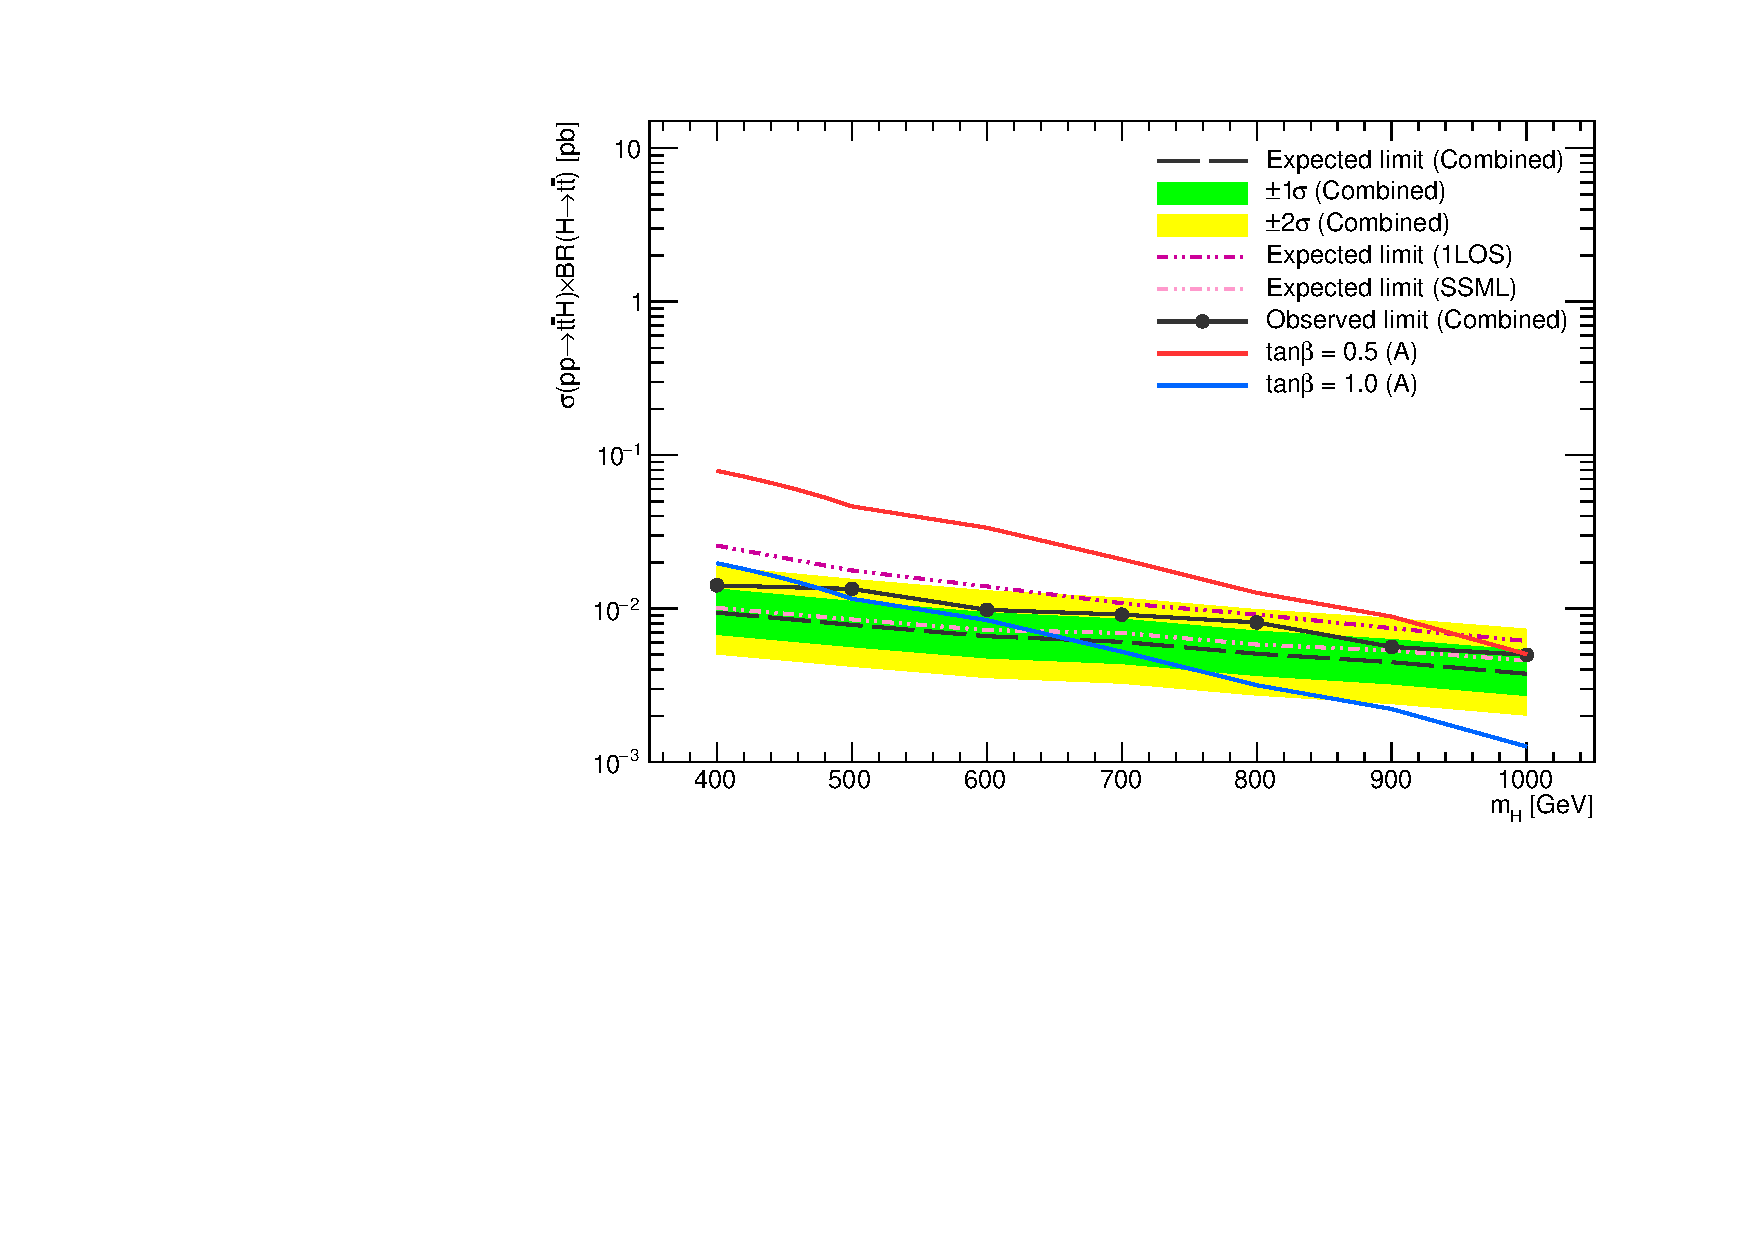
\includegraphics[width=1 \textwidth]{figures/combined_fit/lim_combined_3e1o.pdf}
      \caption{Individual expected limits comparison and observed limit}
    \end{subfigure}
    \caption{\label{fig:combination_limit_1}Observed and expected 95\% CL upper limit on the cross section for the production of $t\bar{t}H/A \to t\bar{t}t\bar{t}$ as a function of $m_{H/A}$ for the combined 1LOS+SSML data fit (left) and comparison plot with expected 95\% CL upper limits times branching fraction to $t\bar{t}$ extracted from separated 1LOS and SSML channels (right).}
\end{figure}

\begin{figure}[htbp!]
    \centering
    \begin{subfigure}[t]{0.49\textwidth}
      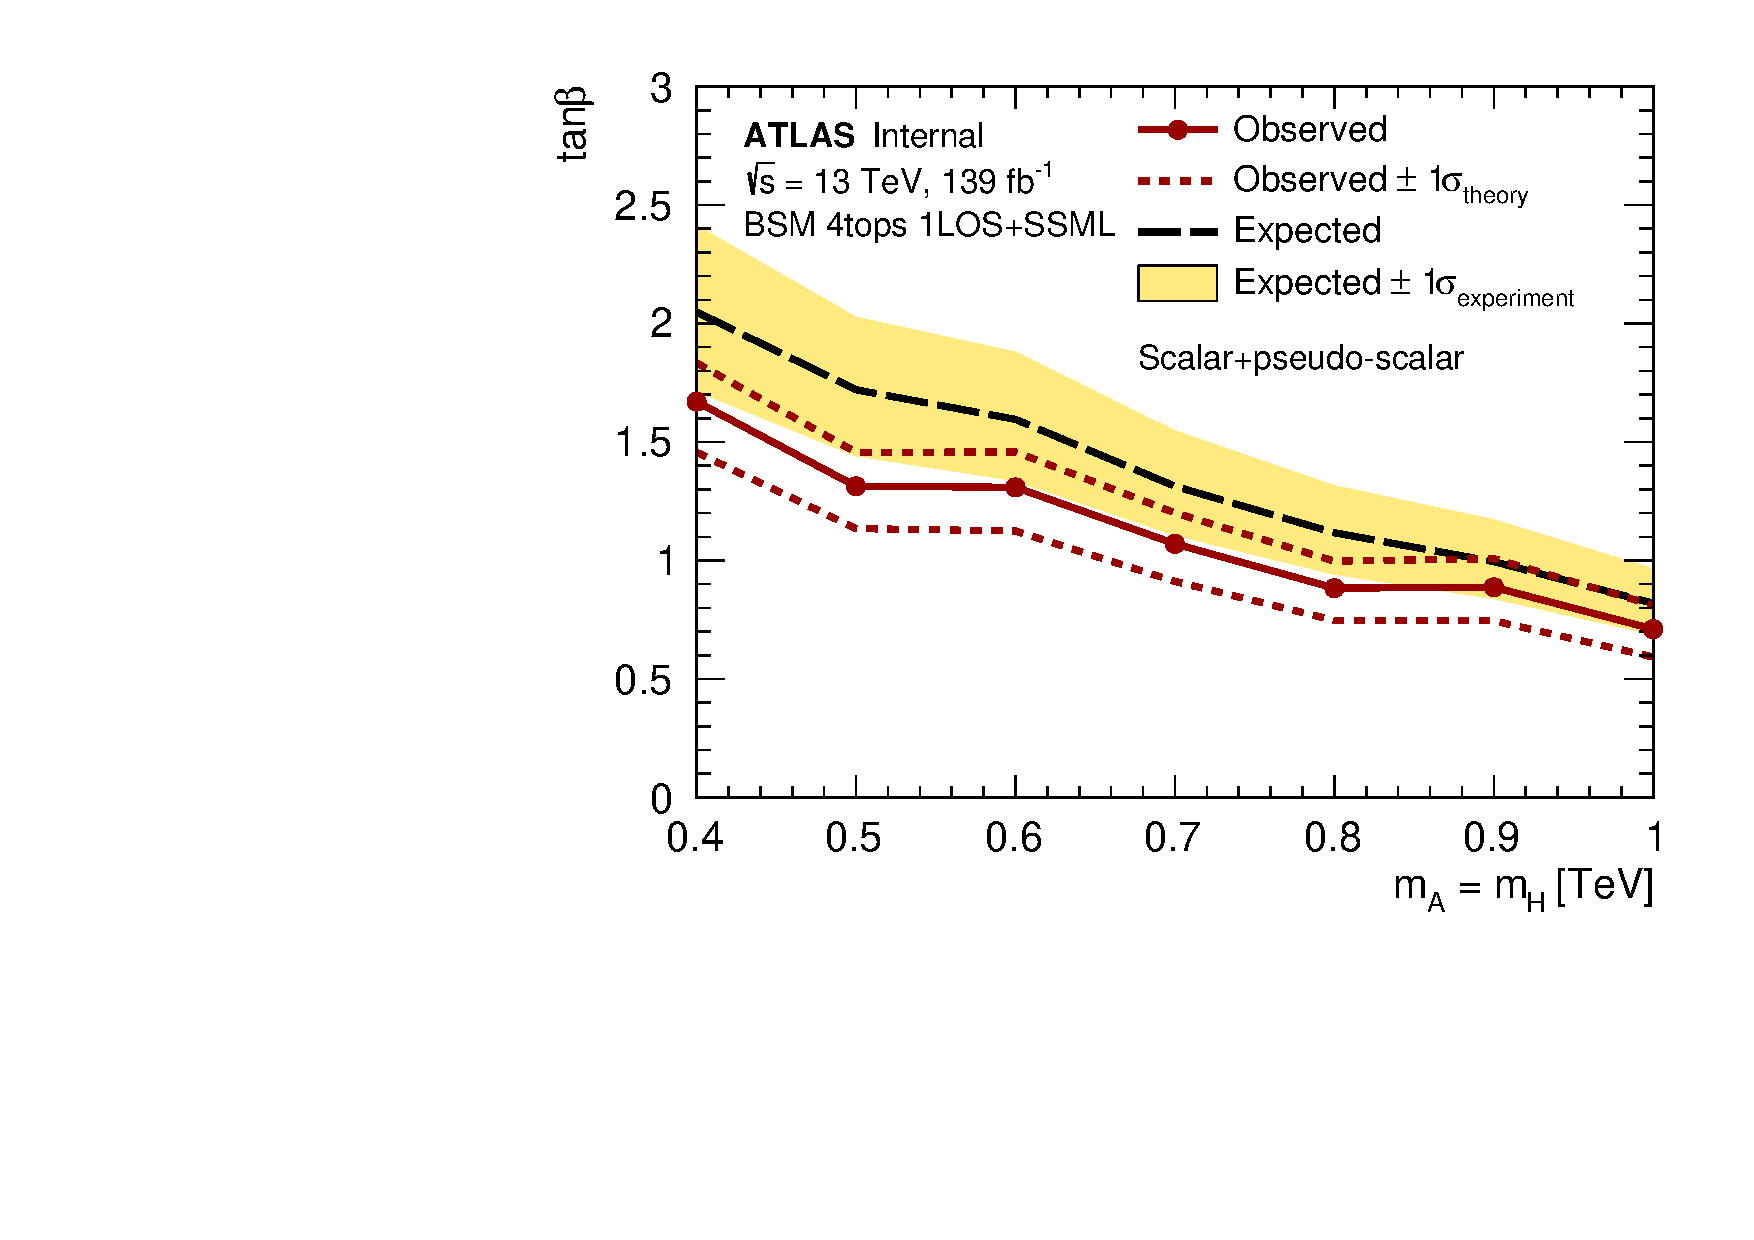
\includegraphics[width=1 \textwidth]{figures/combined_fit/Data_12fb_All.pdf}
      \caption{}
    \end{subfigure}
    \\
    \begin{subfigure}[t]{0.49\textwidth}
      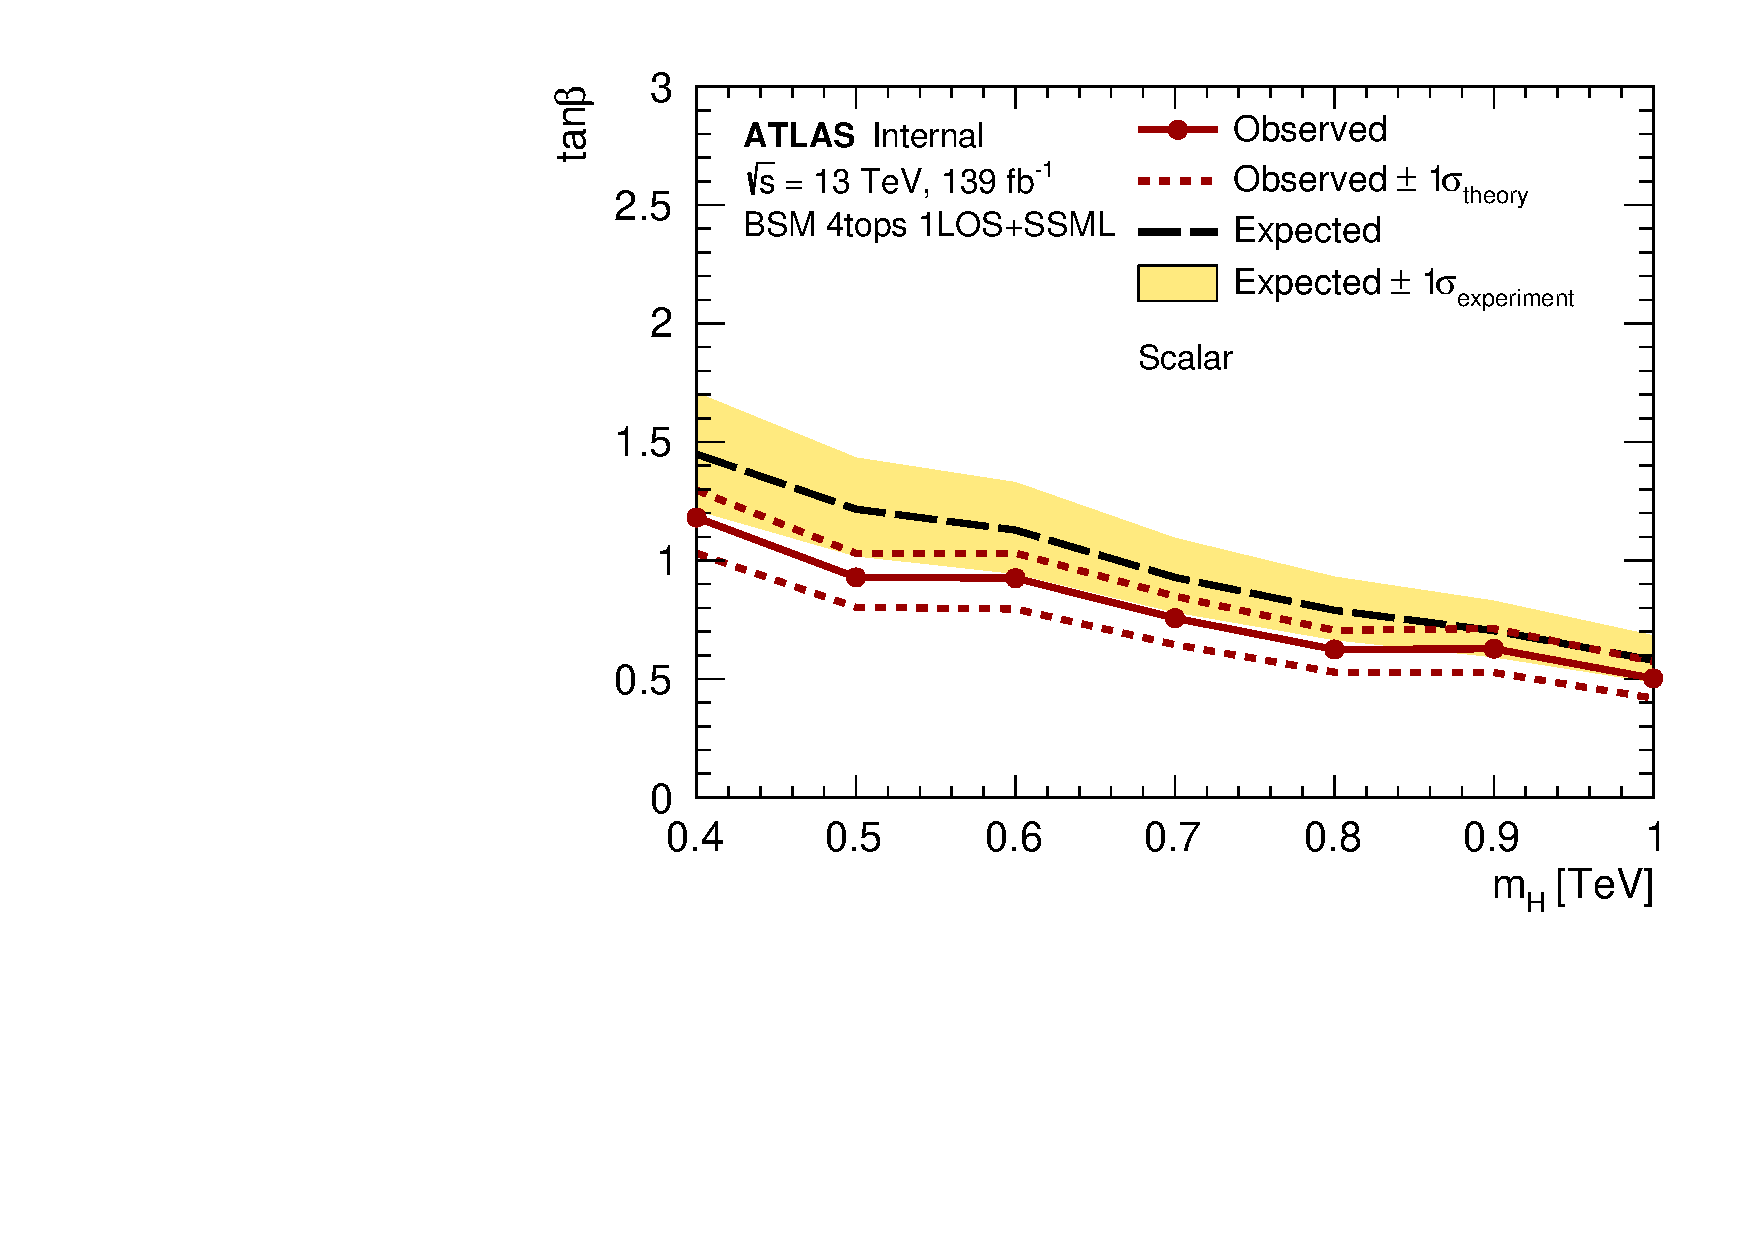
\includegraphics[width=1 \textwidth]{figures/combined_fit/Data_12fb_ttH.pdf}
      \caption{}
    \end{subfigure}
    \begin{subfigure}[t]{0.49\textwidth}
      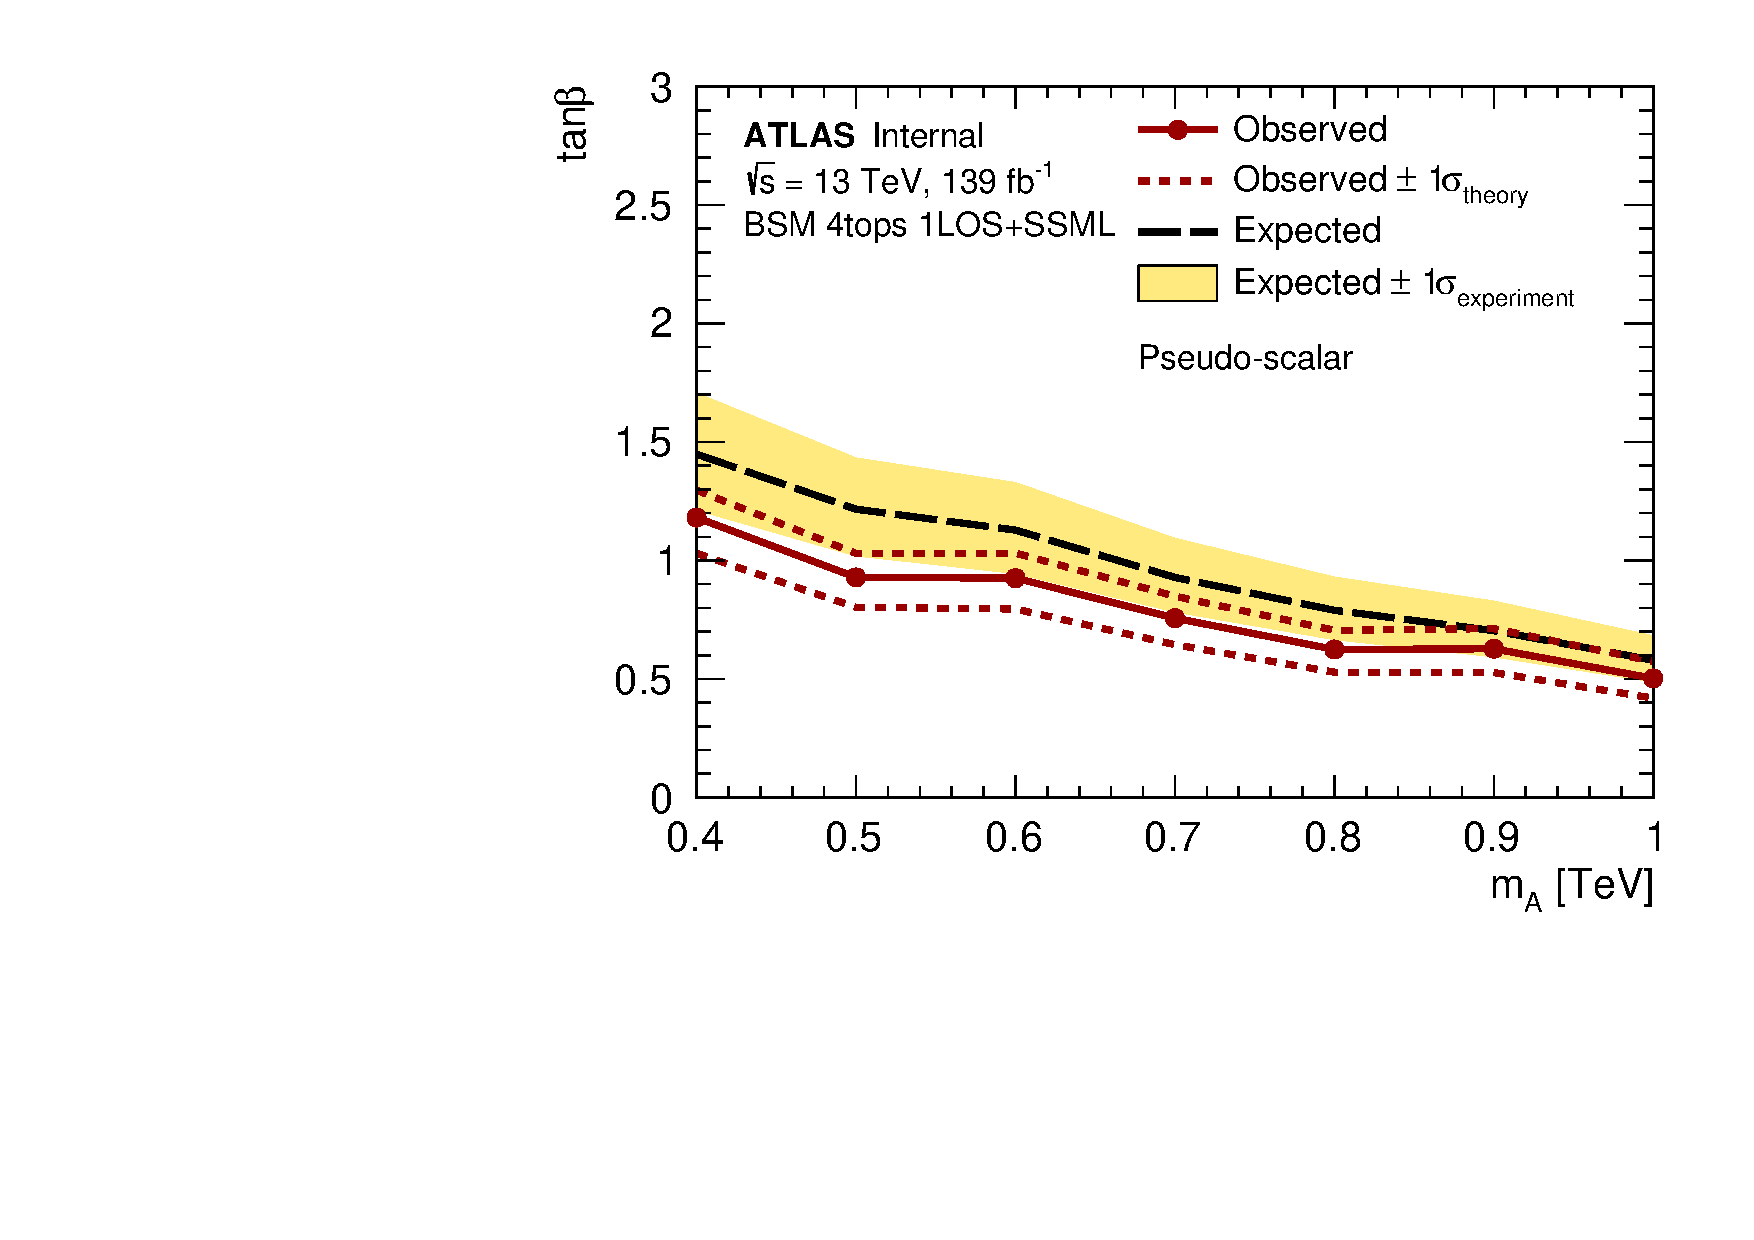
\includegraphics[width=1 \textwidth]{figures/combined_fit/Data_12fb_ttA.pdf}
      \caption{}
    \end{subfigure}
    \caption{\label{fig:combination_2Dplots}Observed and expected exclusion regions at 95$\%$ CL in the $\tan\beta$ versus mass plane assuming that both, a heavy scalar $H$ and pseudo-scalar $A$, contribute to the $t\bar{t}t\bar{t}$ final state and have the same mass $m_{H}=m_{A}$ (a), or assuming that only the scalar $H$ (b) or the pseudo-scalar $A$ contributes (c). The yellow band shows the $\pm1\sigma$ variation on the expected exclusion region. The region below the red solid line is excluded at 95$\%$ CL. The exclusion regions are derived in the context of 2HDM type-II.}
\end{figure}

\begin{figure}
    \centering
    \begin{subfigure}[t]{0.49\textwidth}
      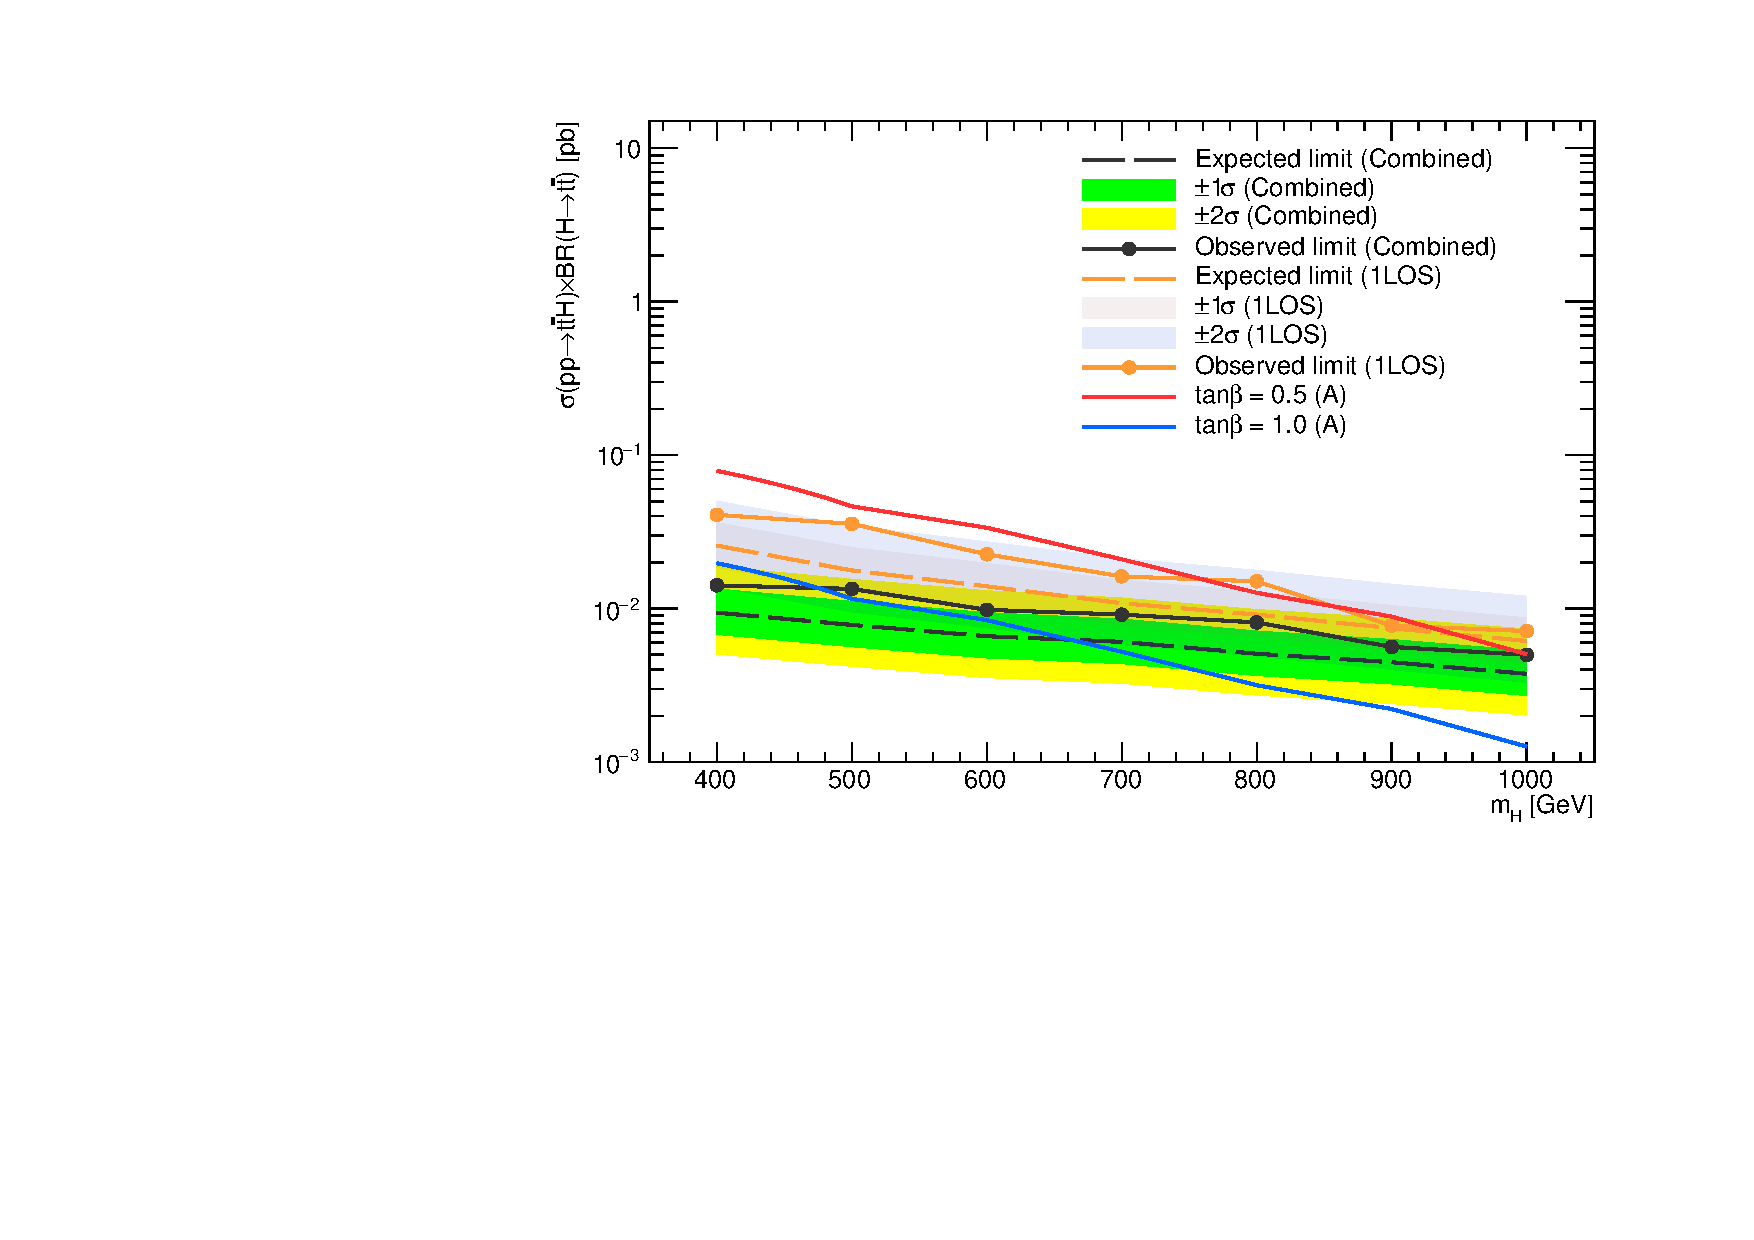
\includegraphics[width=1 \textwidth]{figures/combined_fit/lim_combined_C1.pdf}
      \caption{Comparison between combined and 1LOS}
    \end{subfigure}
    \begin{subfigure}[t]{0.49\textwidth}
      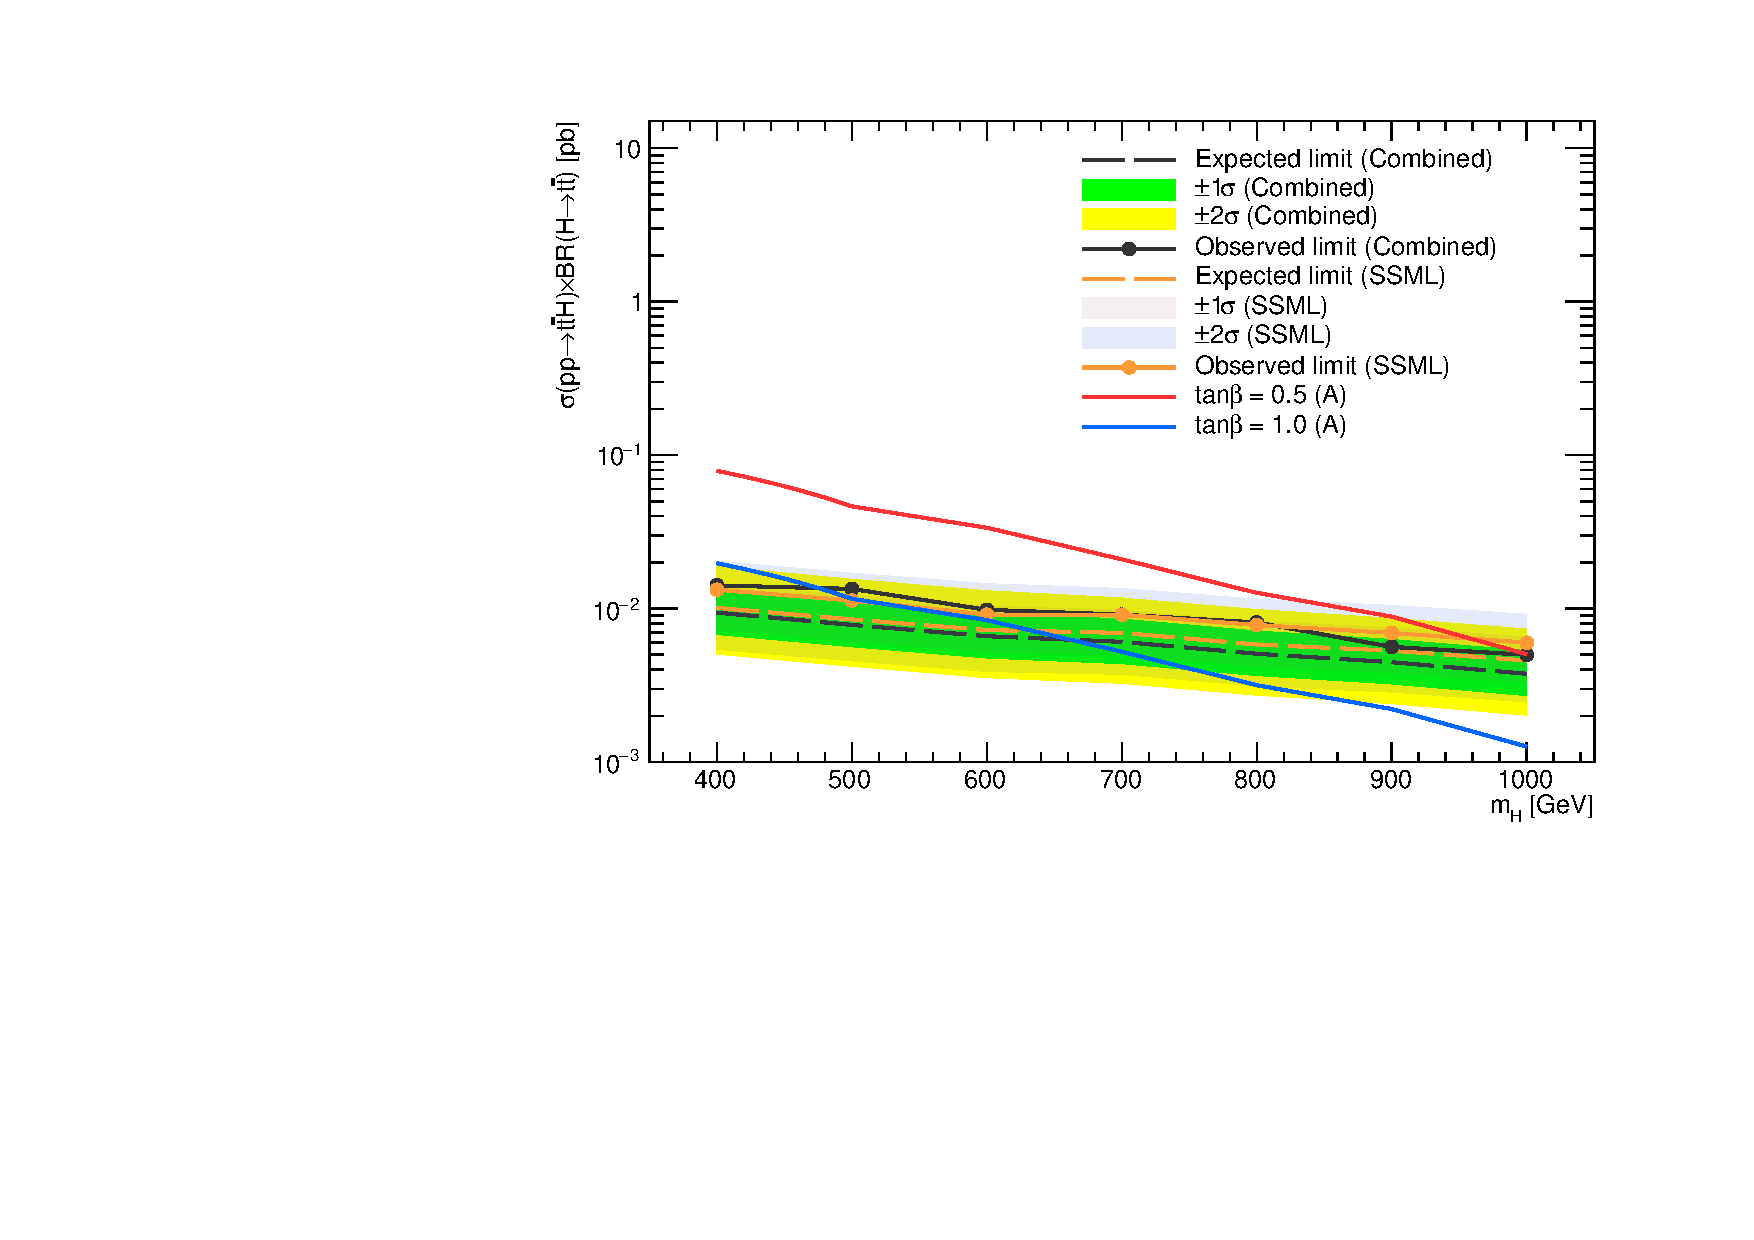
\includegraphics[width=1 \textwidth]{figures/combined_fit/lim_combined_CM.pdf}
      \caption{Comparison between combined and SSML}
    \end{subfigure}
    \caption{\label{fig:combination_limit_2}Comparison of the observed and expected 95\% CL upper limits on the cross section between the combined fit and 1LOS (SSML) channel fit on the right (left).}
\end{figure}

\begin{figure}
    \centering
    \begin{subfigure}[t]{0.49\textwidth}
      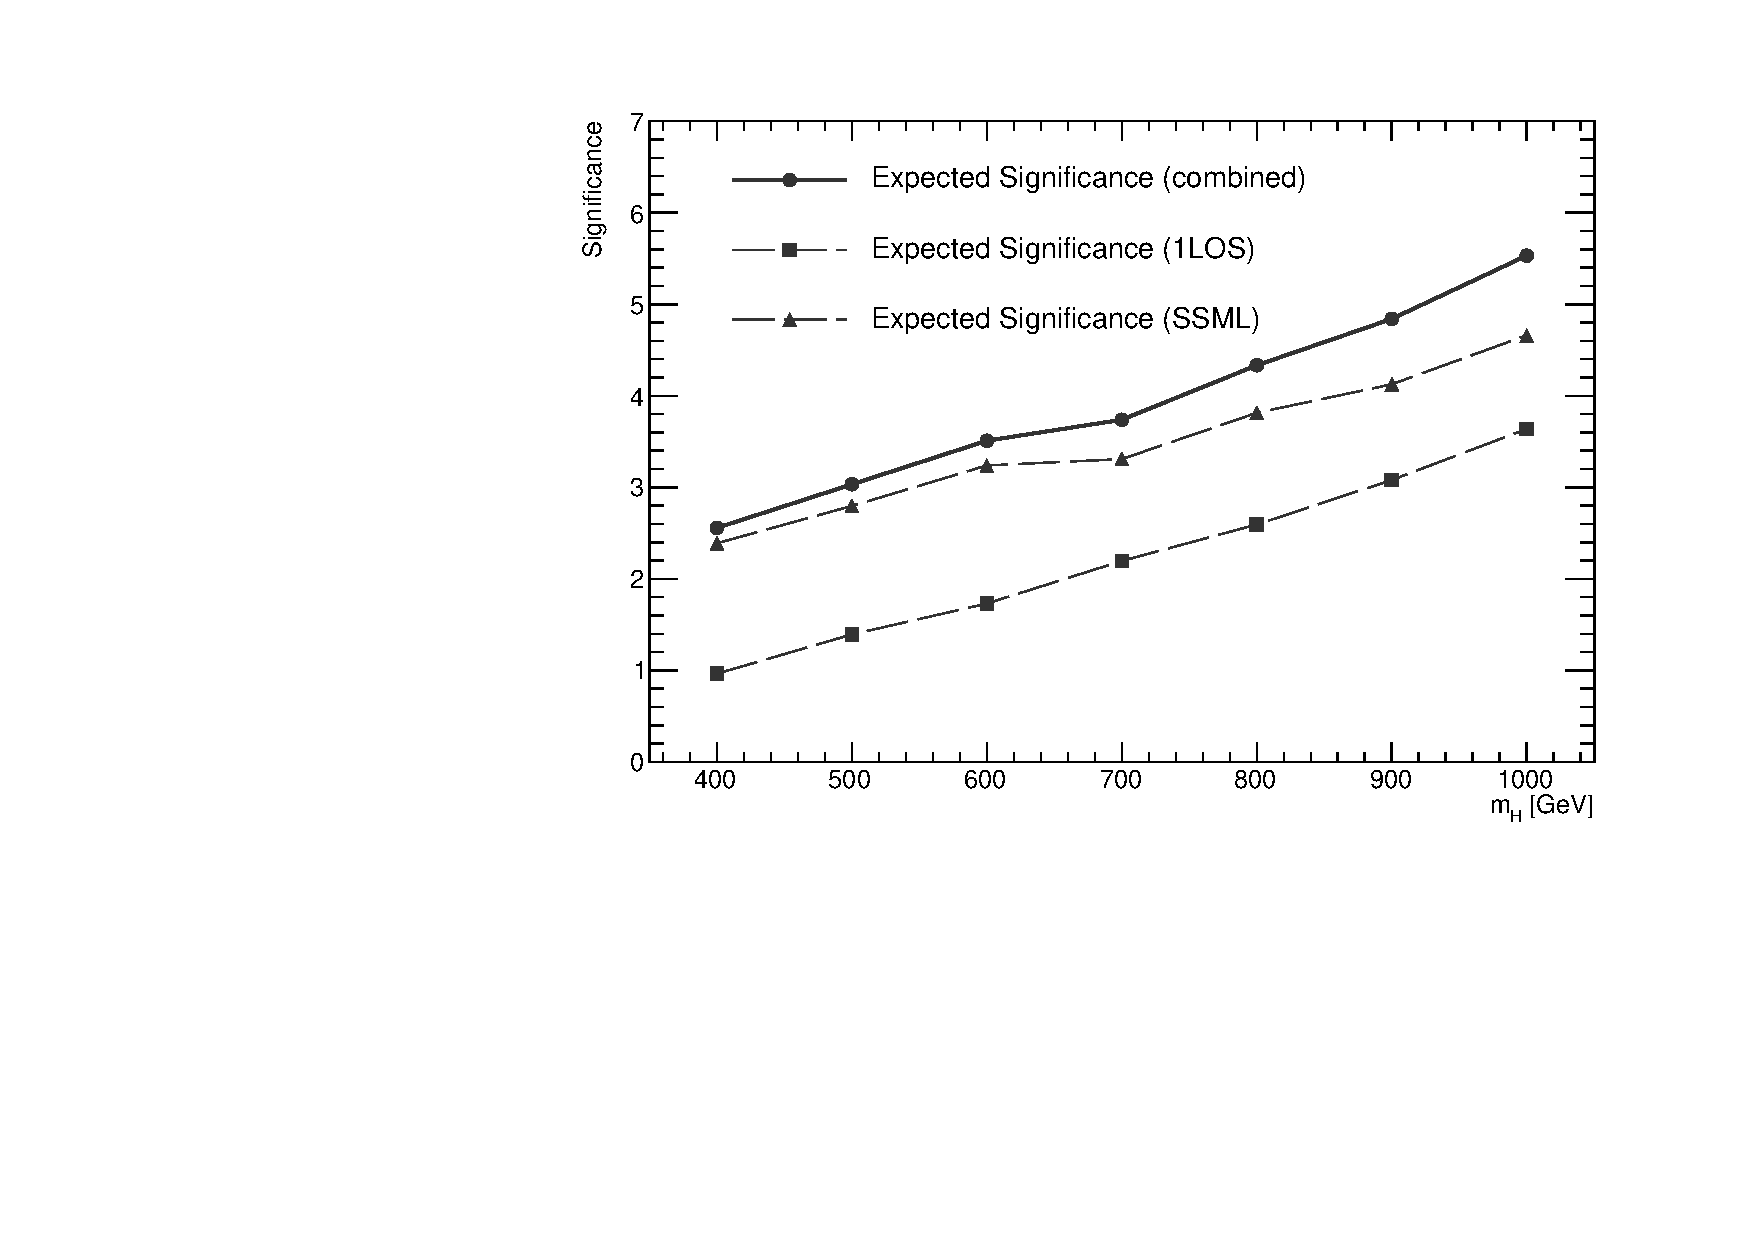
\includegraphics[width=1 \textwidth]{figures/combined_fit/sig_comp_exp.pdf}
      \caption{Expected significance}
    \end{subfigure}
    \begin{subfigure}[t]{0.49\textwidth}
      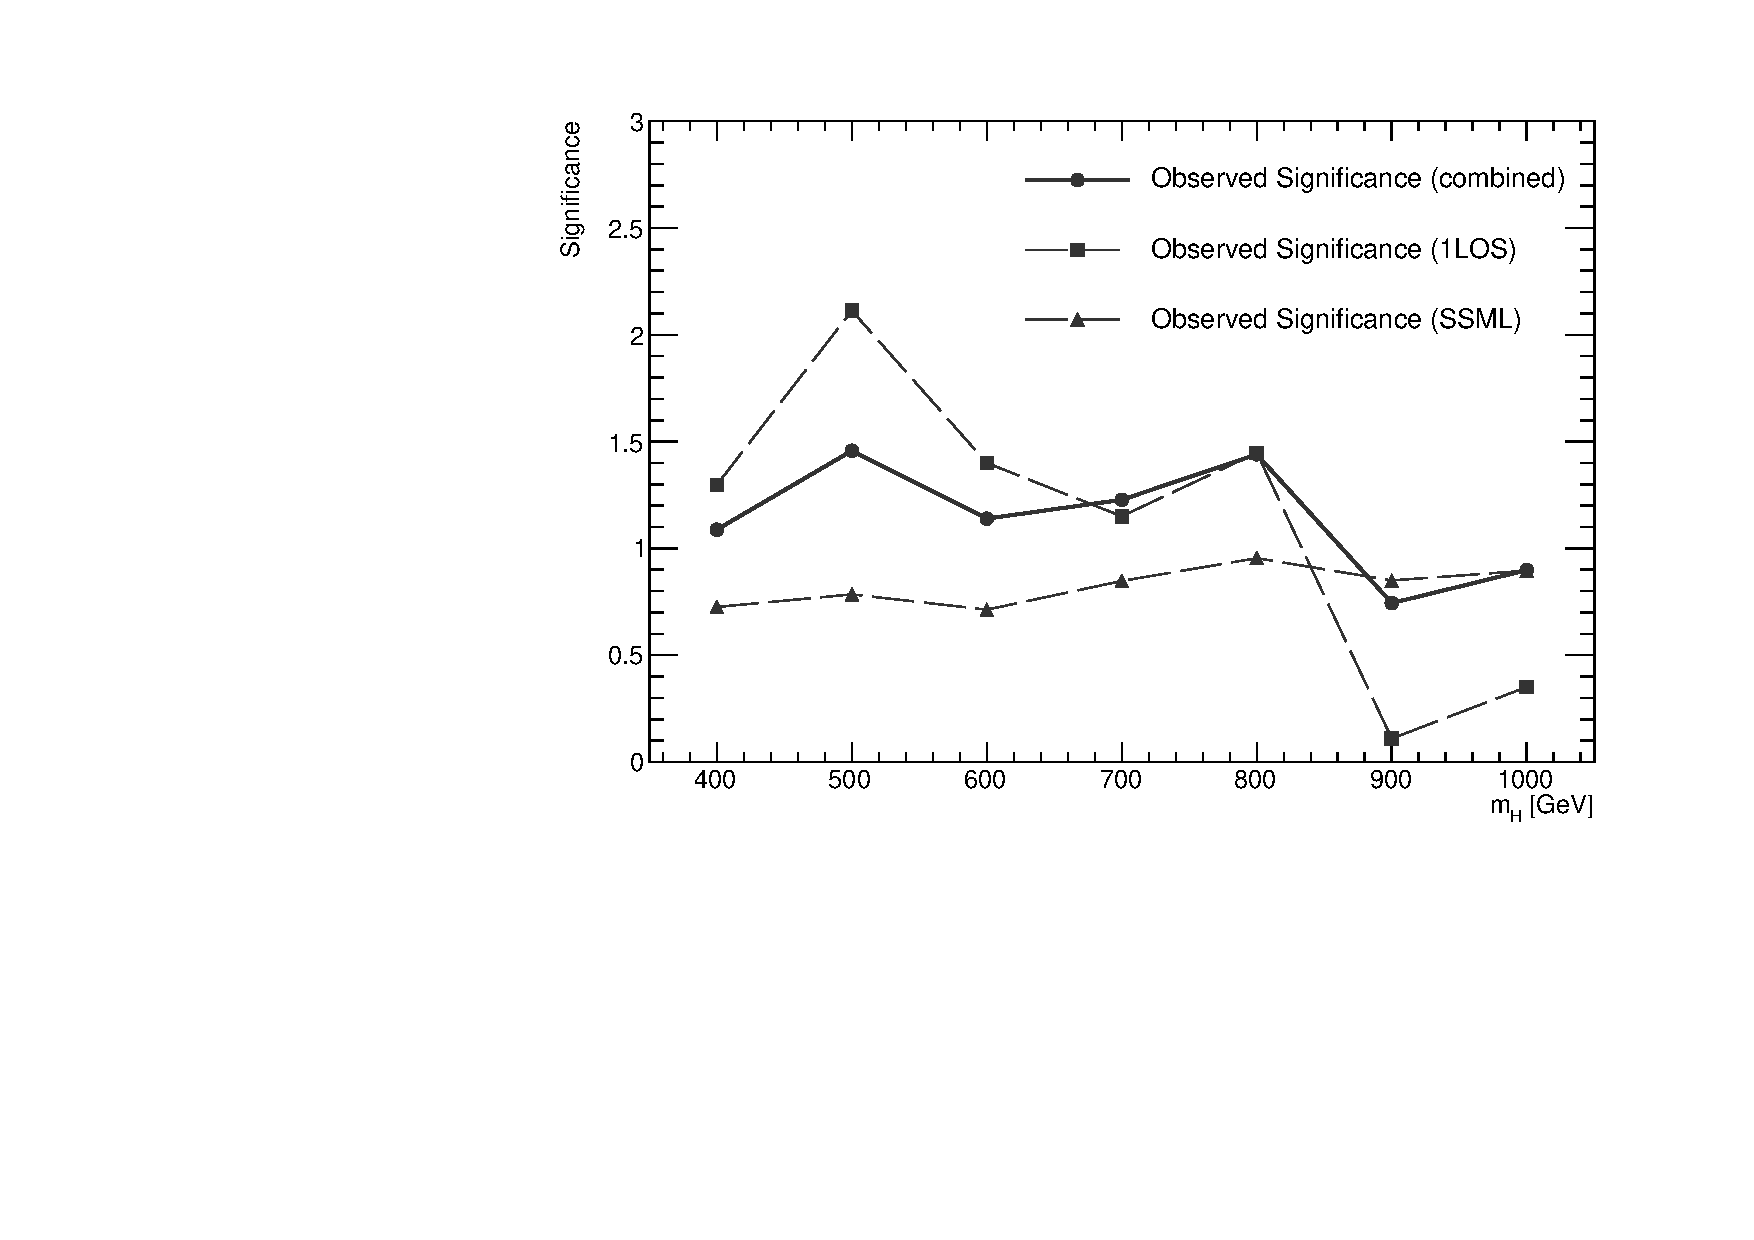
\includegraphics[width=1 \textwidth]{figures/combined_fit/sig_comp_obs.pdf}
      \caption{Observed signifiance}
    \end{subfigure}
    \caption{\label{fig:combination_significance}Comparison of the expected (left) and observed (right) significance among the combined fit and each channel fit.}
\end{figure}

\begin{figure}
    \centering
    \begin{subfigure}[t]{0.49\textwidth}
      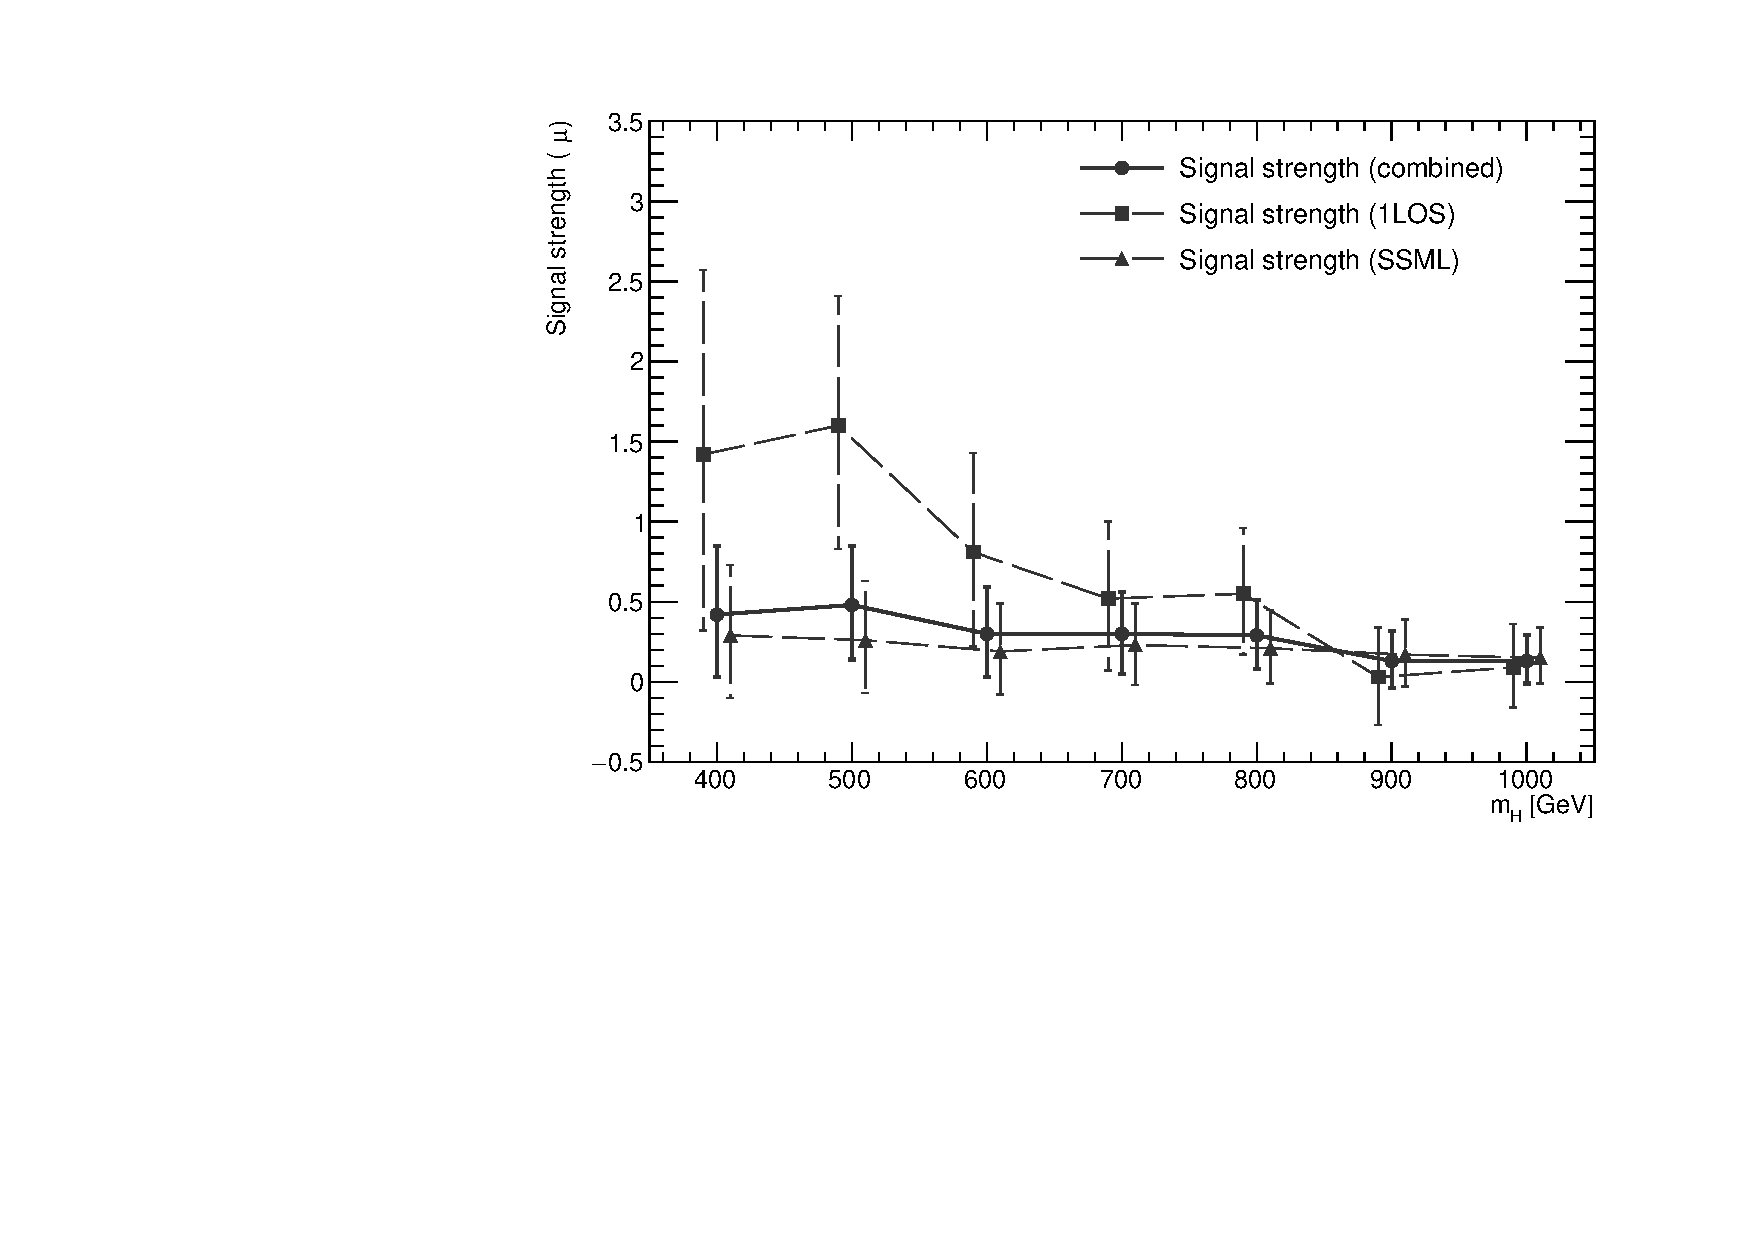
\includegraphics[width=1 \textwidth]{figures/combined_fit/mu_comp.pdf}
      \caption{Signal strenth}
    \end{subfigure}
    \caption{\label{fig:combination_mu}Comparison of the fitted signal strength among the combined fit and each channel fit.}
\end{figure}

\begin{figure}

    \begin{center} \setlength{\tabcolsep}{2.5pt}\footnotesize
    \begin{tabular}{cccc}

    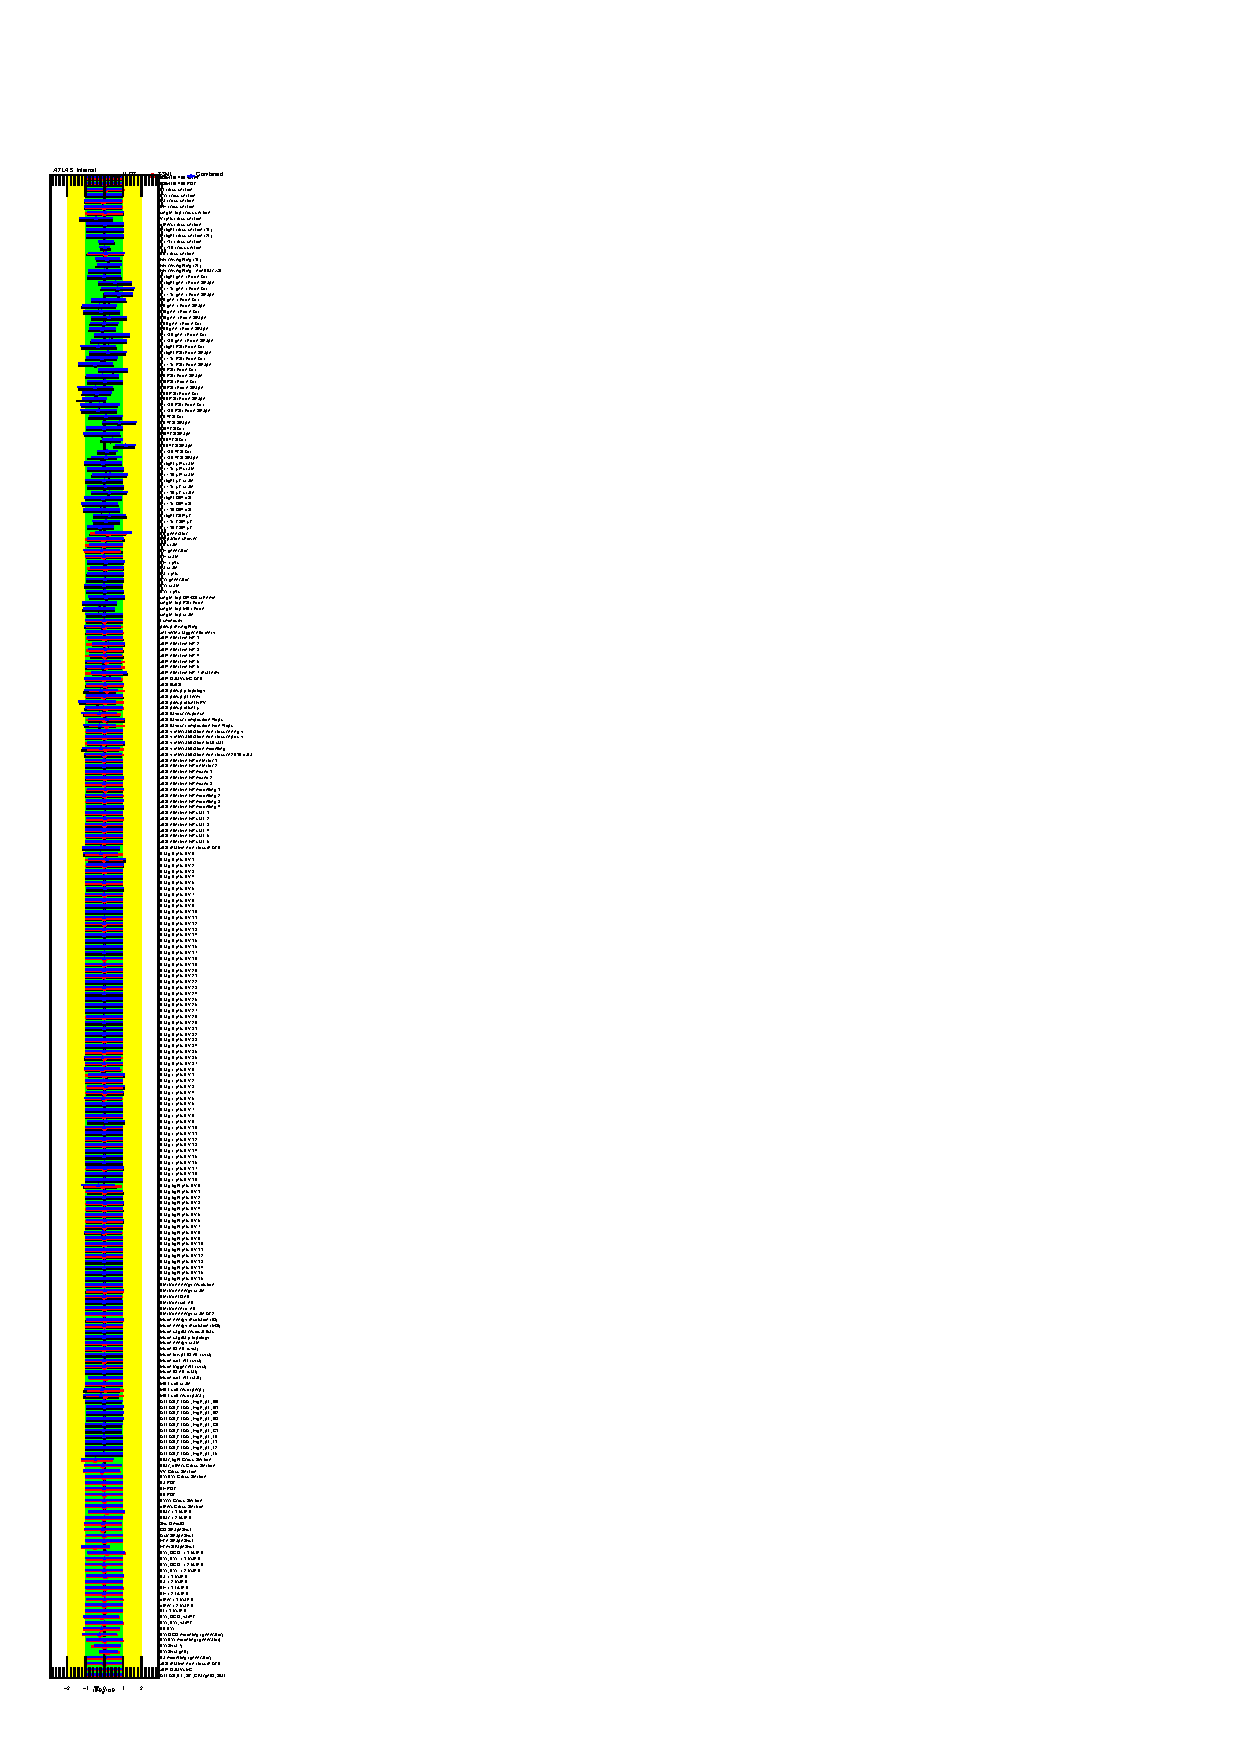
\includegraphics[width=0.2 \textwidth]{figures/combined_fit/NuisPar_comp_400.pdf} &
    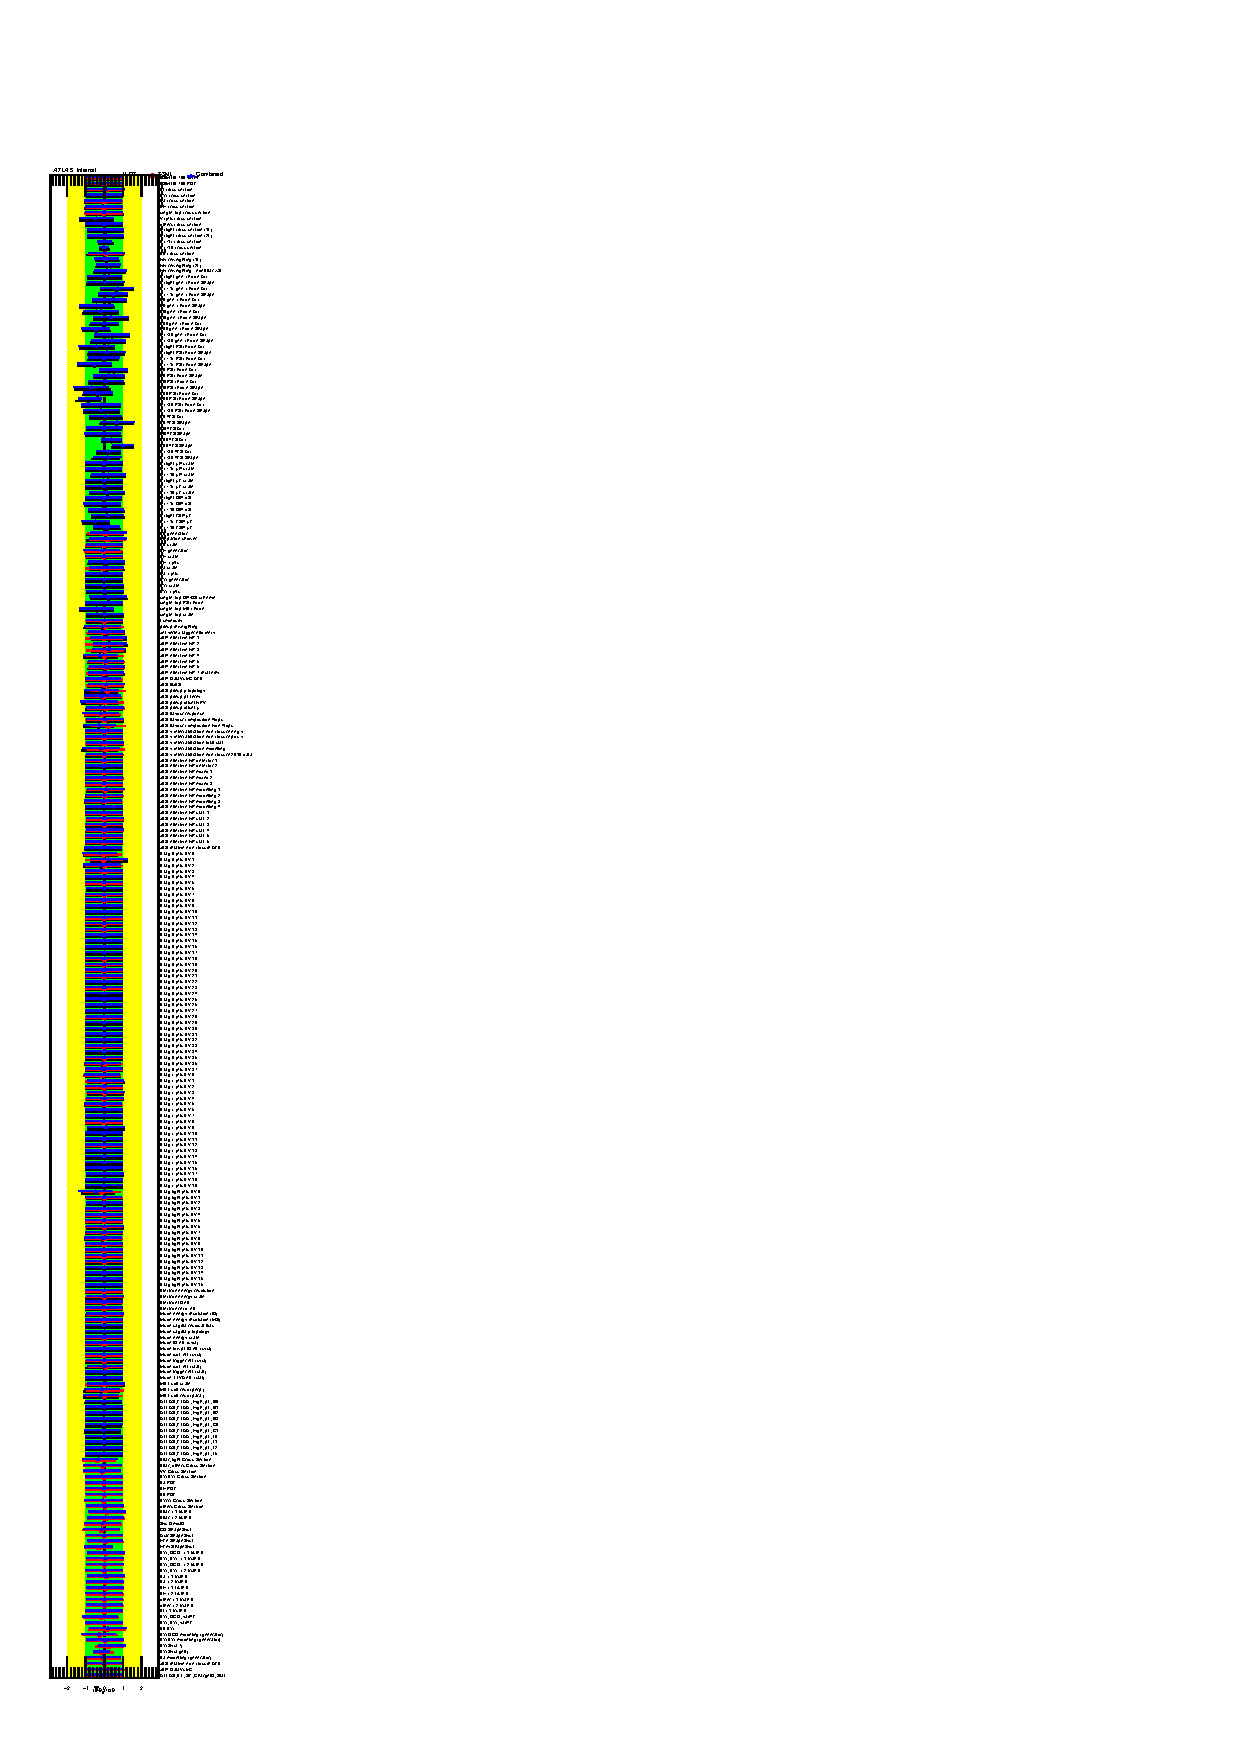
\includegraphics[width=0.2 \textwidth]{figures/combined_fit/NuisPar_comp_700.pdf} &
    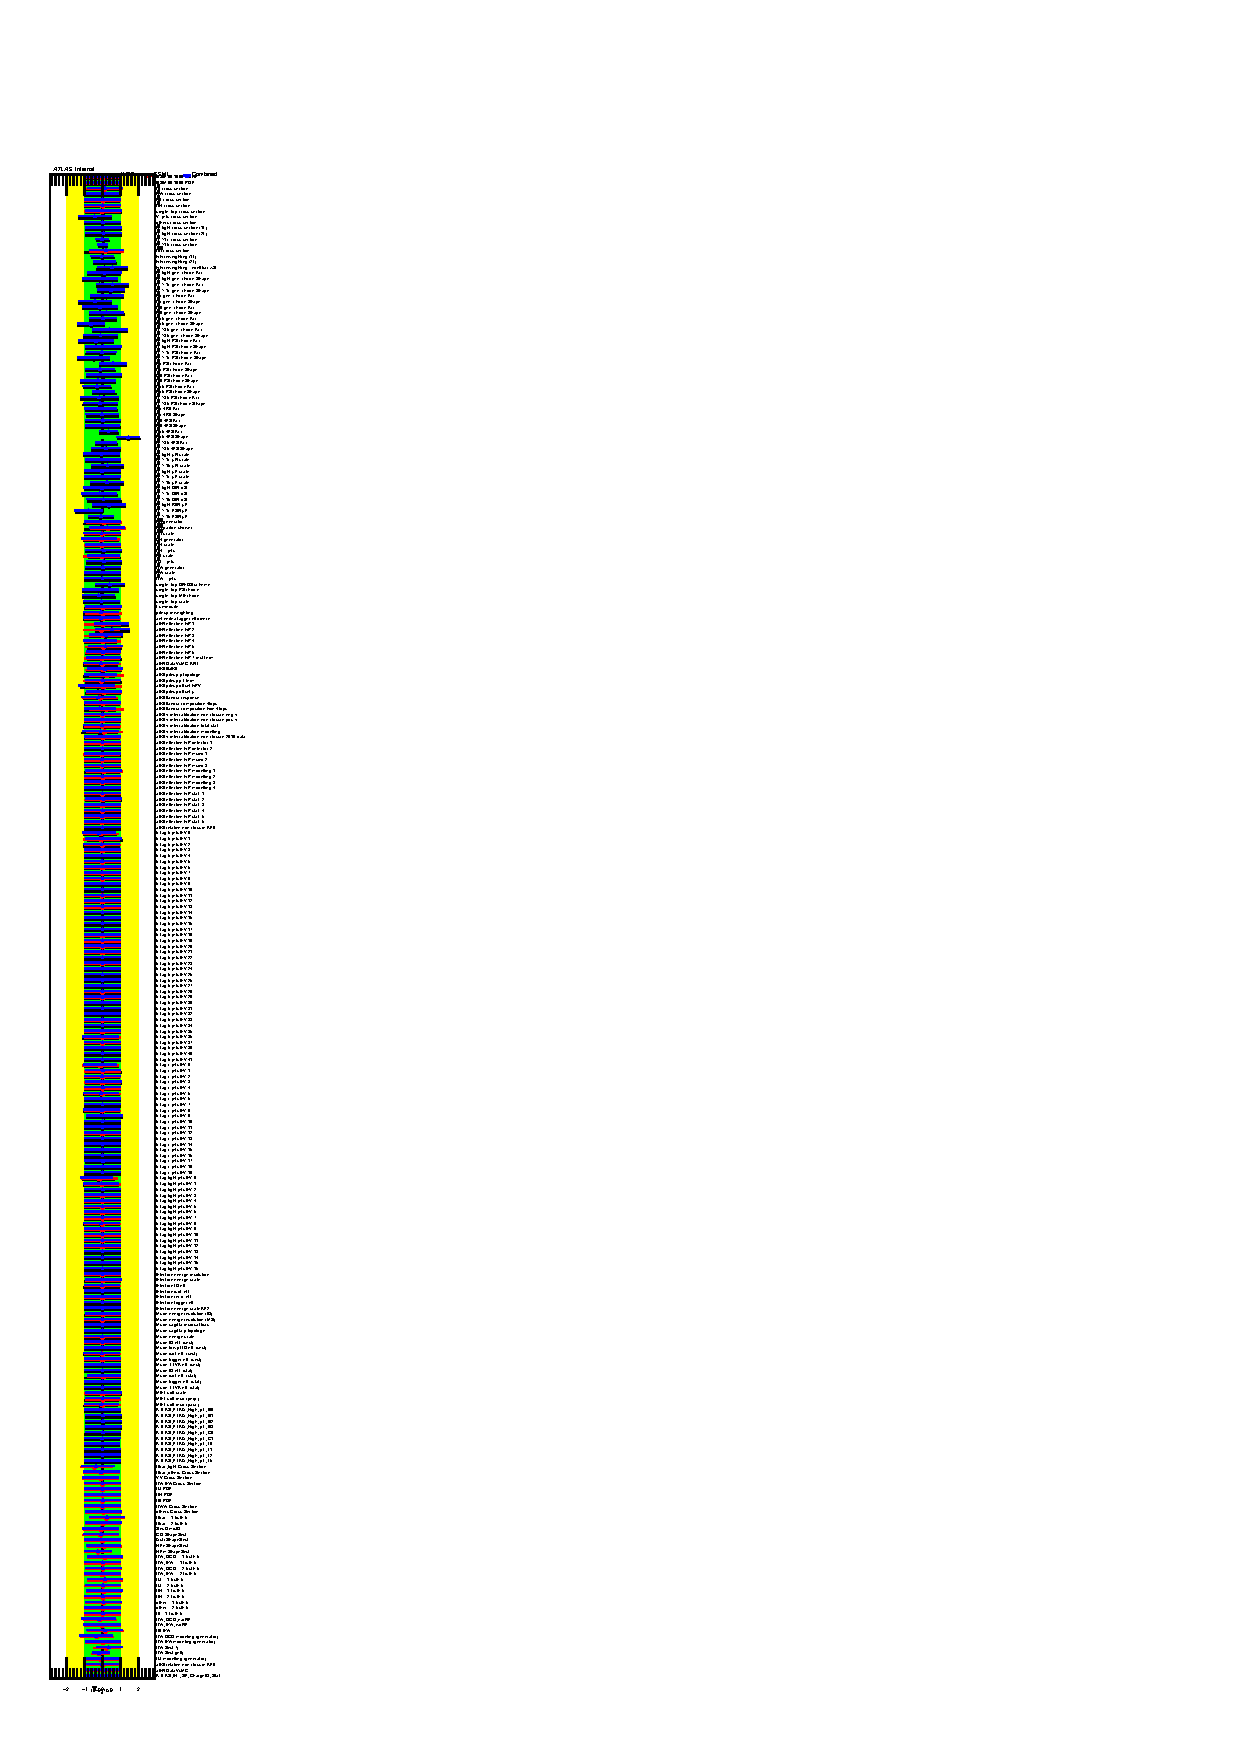
\includegraphics[width=0.2 \textwidth]{figures/combined_fit/NuisPar_comp_1000.pdf}\\

    \end{tabular}
    \end{center}

\caption{\label{fig:combination_NP}Nuisance parameter pulls and constraints among the combined fit and each channel fit at mass point 400 GeV (left), 700 GeV (middle), 1000 GeV (right).}
\end{figure}

\begin{figure}

    \begin{center} \setlength{\tabcolsep}{2.5pt}\footnotesize
    \begin{tabular}{cccc}

    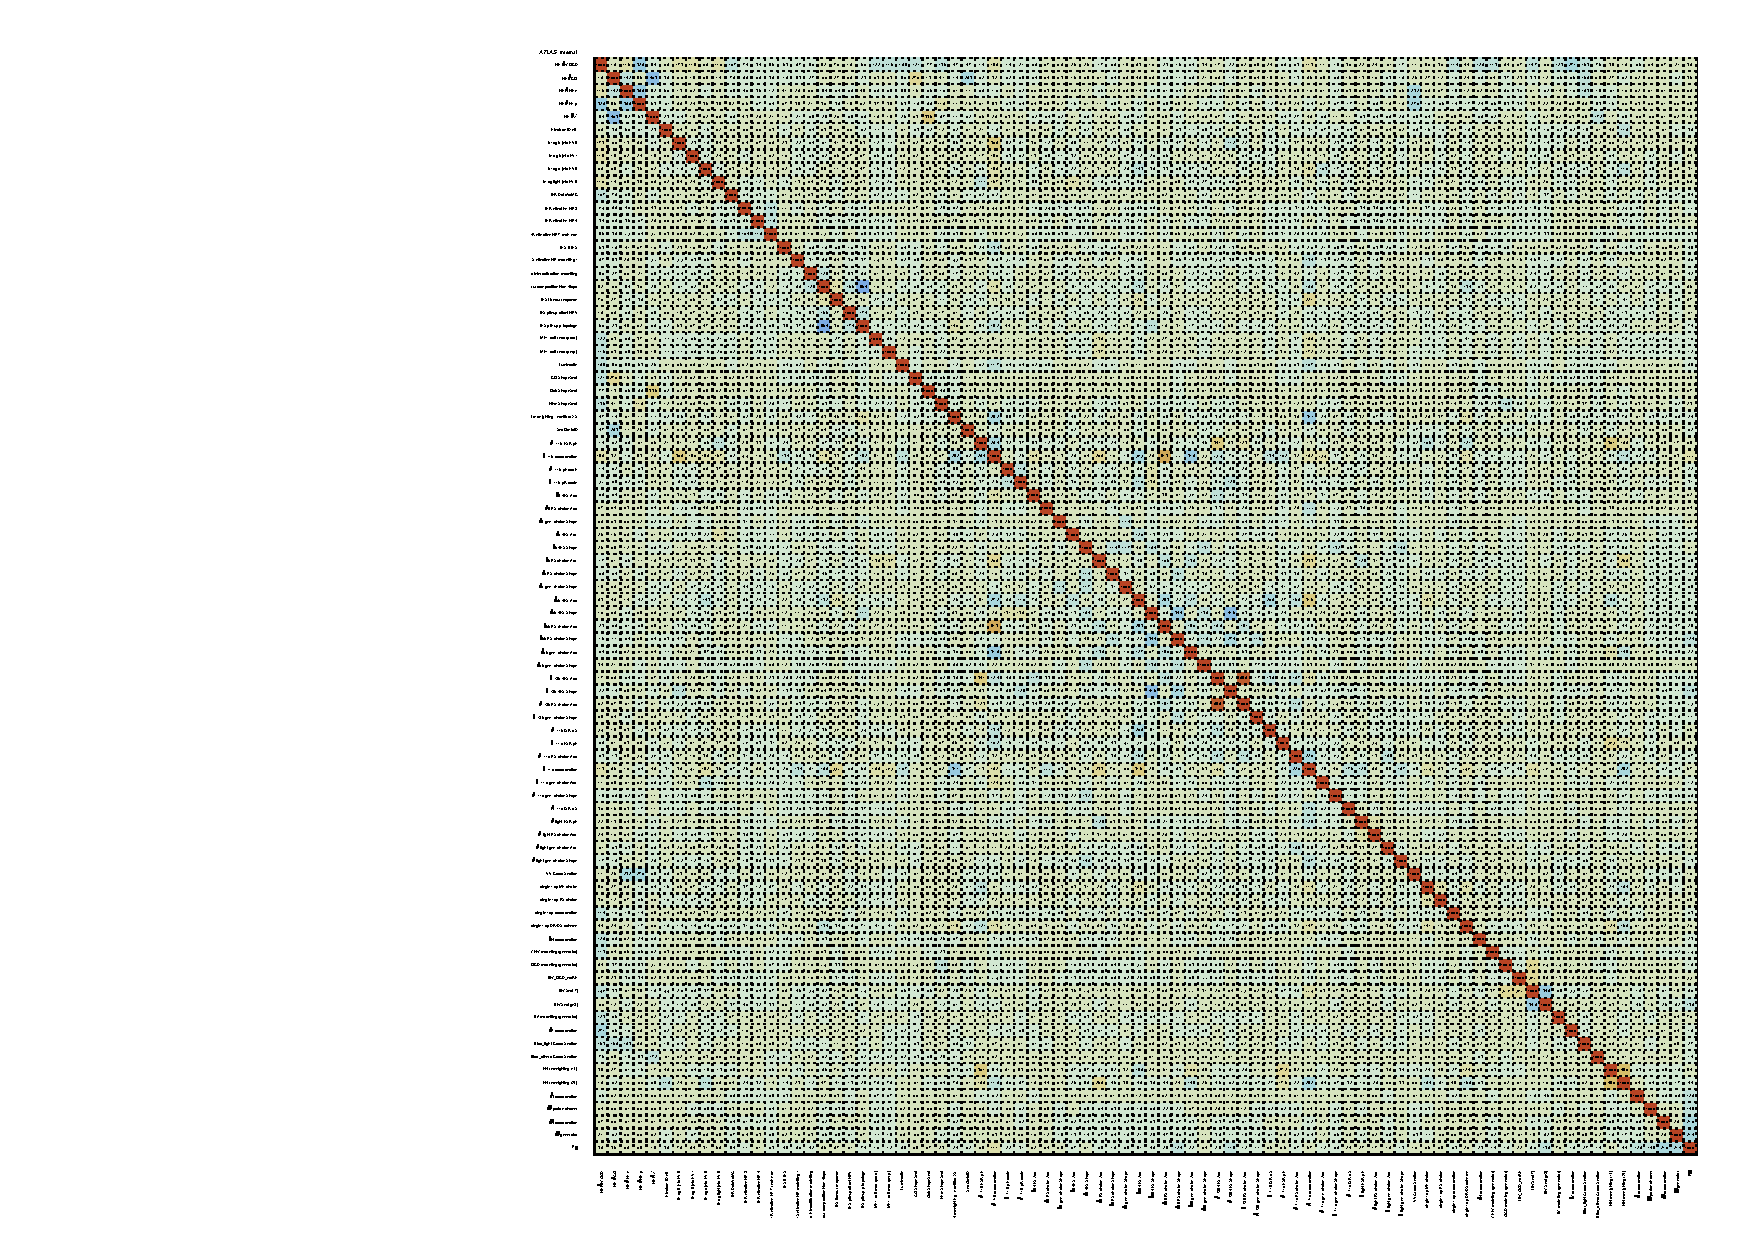
\includegraphics[width=0.95 \textwidth]{figures/combined_fit/CorrMatrix_comb_400.pdf}\\

    \end{tabular}
    \end{center}

\caption{\label{fig:combination_CorrMatrix}Correlation Matrix of combined data fit at mass point 400 GeV.}
\end{figure}